\documentclass[11pt]{article}
\usepackage{geometry, titlesec}
\usepackage[parfill]{parskip}
\usepackage[italicdiff]{physics}
\usepackage{amsfonts, amsthm, mathrsfs}
\usepackage[cm]{fullpage}
\usepackage{fancyhdr}
\usepackage{enumitem}
\usepackage{xcolor, soul}
\usepackage{siunitx}
\allowdisplaybreaks

\renewcommand{\thesubsection}{\thesection.\alph{subsection}}
%\renewcommand{\vb}[1]{\mathbf{#1}}
\newcommand{\vfix}{\vspace{-\baselineskip}}

\makeatletter
\renewcommand*\env@cases[1][1.2]{%
  \let\@ifnextchar\new@ifnextchar
  \left\lbrace
  \def\arraystretch{#1}%
  \array{@{}l@{\quad}l@{}}%
}
\makeatother
 
\renewcommand{\footrulewidth}{.2pt}
%\setlist[enumerate]{leftmargin=*}
\pagestyle{fancy}
\fancyhf{}
\lhead{\textbf{Physics 322 Homework 3}}
\rhead{Lacey Rainbolt}
\setlength{\headheight}{11pt}
\setlength{\headsep}{11pt}
\setlength{\footskip}{24pt}
\lfoot{\today}
\rfoot{\thepage}

\titleformat{\section}[runin]{\normalfont\large\bfseries}{Problem \thesection.}{1em}{}
\titleformat{\subsection}[runin]{\normalfont\large\bfseries}{\thesubsection}{1em}{}
\titleformat{\subparagraph}[leftmargin]{\normalfont\normalsize\bfseries}{}{0pt}{}

\newcommand{\refeq}[1]{(\ref{#1})}

\newcommand{\beq}{\begin{equation*}}
\newcommand{\eeq}{\end{equation*}}

\newcommand{\beqn}{\begin{equation}}
\newcommand{\eeqn}{\end{equation}}

\newcommand{\blg}{\begin{align*}}
\newcommand{\elg}{\end{align*}}


\newenvironment{statement}[1]
{
	\section{#1}
	\color{darkgray}
	\ignorespaces
}
{
%    \smallskip
}

\newenvironment{problem}
{
	\subsection{}
	\color{darkgray}
%	\paragraph{Problem.}
    \ignorespaces
}
{

}

\newenvironment{solution}
{
    \paragraph{Solution.}
    \ignorespaces
}
{
    \bigskip
}



\begin{document}

\newcommand{\eps}{\epsilon}
\newcommand{\vx}{\vb{x}}
\newcommand{\phix}{\phi(\vx)}
\newcommand{\dcx}{\dd[3]{x}}
\newcommand{\dcxp}{\dd[3]{x'}}
\newcommand{\rhox}{\rho(\vx)}
\newcommand{\rhoxp}{\rho(\vx')}
\newcommand{\rhopxp}{\rho'(\vx')}
\newcommand{\xh}{\vec{\hat{x}}}
\newcommand{\absx}{\abs{\vx}}
\newcommand{\absxp}{\abs{\vx'}}

\newcommand{\Ylm}{Y_{l m}}
\newcommand{\qlm}{q_{l m}}
\newcommand{\Plm}{P_l^m}
\newcommand{\tht}{\theta}
\newcommand{\cost}{\cos\tht}
\newcommand{\vph}{\varphi}
\newcommand{\tv}{(\tht, \vph)}
\newcommand{\tvp}{(\tht', \vph')}
\newcommand{\Gxxp}{G(\vx, \vx')}
\newcommand{\Gpxxp}{G'(\vx, \vx')}
\newcommand{\Gdxxp}{G_D(\vx, \vx')}
\newcommand{\qplm}{q'_{l m}}

\newcommand{\lap}{\nabla^2}
\newcommand{\evphi}{\ev{\phi}}
\newcommand{\evphix}{\evphi\!(\vx)}
\newcommand{\rhof}{\rho_f}
\newcommand{\evrhof}{\ev{\rhof}}
\newcommand{\fe}{\frac{1}{\eps}}
\newcommand{\tif}{\text{if }}
\newcommand{\Al}{A_l}
\newcommand{\Bl}{B_l}
\newcommand{\Cl}{C_l}

\newcommand{\intoi}{\int_0^\infty}
\newcommand{\intono}{\int_{-1}^{1}}
\newcommand{\intotp}{\int_0^{2\pi}}
\newcommand{\drp}{\dd{r'}}
\newcommand{\dctp}{\dd{(\cost')}}
\newcommand{\dvp}{\dd{\vph'}}

\newcommand{\Ylotv}{Y_{l 0}\tv}
\newcommand{\dr}{\dd{r}}
\newcommand{\dct}{\dd{(\cost)}}
\newcommand{\ddv}{\dd{\vph}}

\newcommand{\Alm}{A_{l m}}
\newcommand{\Blm}{B_{l m}}
\newcommand{\Ploct}{P_l^0(\cost)}
\newcommand{\Ploctp}{P_l^0(\cost')}
\newcommand{\alp}{\alpha}
\newcommand{\rtp}{(r, \tht, \phi)}
\newcommand{\phirtp}{\phi\rtp}
\newcommand{\qlo}{q_{l 0}}
\newcommand{\qplo}{q'_{l 0}}
\newcommand{\qpplm}{q''_{l m}}
\newcommand{\qpplo}{q''_{l 0}}

\newcommand{\vD}{\vb{D}}
\newcommand{\evD}{\ev{\vD}}
\newcommand{\nh}{\vb{\hat{n}}}
\newcommand{\vE}{\vb{E}}
\newcommand{\evE}{\ev{\vE}}
\newcommand{\Er}{E_r}
\newcommand{\evEr}{\ev{\Er}}
\newcommand{\rh}{\vb{\hat{r}}}

\newcommand{\dint}{\displaystyle \int}
\newcommand{\dsum}{\displaystyle \sum}

\begin{statement}{} \label{1}
	Consider a dielectric ball of radius $R$ with dielectric constant $\eps$.  Obtain a multipole expansion for the field, $\phix$, of a point charge $q$ placed at a point $\vx'$ with $\abs{\vx'} = d > R$ (so the charge is outside of the dielectric ball).
	
	Hint: Follow the procedure we used in class to find the multipole expansion of a point charge without the dielectric, but now consider the three regions $r \leq R$, $R \leq r \leq d$, and $r \geq d$.  Obtain the form of the solution in these regions and match suitably.
\end{statement}

\begin{solution}
	In class, we derived the multipole expansion for $\absx \geq R$ when the charge distribution $\rhoxp$ is nonzero only within $\abs{\vx'} \leq R$.  We can find an equivalent expression for the reverse situation (within $\absx \leq R$ when the charge distribution $\rhoxp$ is nonzero only for $\abs{\vx'} \geq R$) using the spherical harmonic expansion of the Green's function $\Gxxp$ in Eq.~(2.78):
	\beqn \label{greenexp}
		\Gxxp = \frac{1}{\abs{\vx - \vx'}}
		= \begin{cases}
			\dsum_{l,m} \dfrac{4\pi}{2l + 1} \dfrac{r^l}{{r'}^{l + 1}} \Ylm^*\tvp \, \Ylm\tv & \tif r < r', \\[2ex]
			\dsum_{l,m} \dfrac{4\pi}{2l + 1} \dfrac{{r'}^l}{r^{l + 1}} \Ylm^*\tvp \, \Ylm\tv & \tif r > r'.
		\end{cases}
	\eeqn
	As in Eq.~(2.79) in the course notes, we integrate and obtain
	\beq
		\phix = \int \Gxxp \, \rhoxp \dcxp
		= \sum_{l, m} \frac{4\pi}{2l + 1} r^l \Ylm\tv \int \frac{\rhoxp}{{r'}^{l+1}} \Ylm^*\tvp \dcxp.
	\eeq
	Combining this with the result of Eq.~(2.79), we have
	\beqn \label{multipole}
		\phix = \begin{cases}
			\dsum_{l, m} \dfrac{4\pi}{2l + 1} r^l \, \qplm \, \Ylm\tv & \tif r < r' \text{ and } \rhoxp(r) = 0, \\[2ex]
			\dsum_{l,m} \dfrac{4\pi}{2l + 1} \dfrac{\qlm}{r^{l+1}} \Ylm\tv & \tif r > r' \text{ and } \rhoxp(r) = 0,
		\end{cases}
	\eeqn
	where
	\begin{align} \label{qlm}
		\qplm &\equiv \int \frac{\rhoxp}{{r'}^{l+1}} \Ylm^*\tvp \dcxp, &
		\qlm &\equiv \int \rhoxp \, {r'}^l \, \Ylm^*\tvp \dcxp,
	\end{align}
	from Eq.~(2.80) and our derivation.
	
	Additionally, the spherical harmonics $\Ylm$ are given by Eq.~(2.58),
	\beq
		\Ylm\tv = \sqrt{\frac{2l + 1}{4\pi}} \sqrt{\frac{(l - m)!}{(l + m)!}} \Plm(\cost) e^{i m \vph},
	\eeq
	and the associated Legendre polynomials $\Plm$ are given by Eq.~(2.59),
	\beq
		\Plm(x) = \frac{(-1)^m}{2^l l!} (1 - x^2)^{m/2} \dv[l + m]{}{x} (x^2 - 1)^l.
	\eeq	
	
	We assume the dielectric is linear, homogeneous, and isotropic.  Poisson's equation inside such a dielectric is given by Eq.~(3.22) in the course notes,
	\beq
		\lap\evphi = -\frac{4\pi}{\eps} \evrhof\!,
	\eeq
	where $\rhof$ is the free charge density.  Here, $\evrhof = 0$ since there are no free charges within the dielectric, so this reduces to Laplace's equation.  The general solution to Laplace's equation is given by Eq.~(3.61) in Jackson,
	\beqn \label{lapsol}
		\evphi\!(r, \tht, \vph) = \sum_{l,m} \left( \Alm r^l + \frac{\Blm}{r^{l+1}} \right) \, \Ylm\tv,
	\eeqn
	where $\Alm$ and $\Blm$ are constant coefficients.
	
	We will begin inside the dielectric, where $r \leq R$.  Here we must have $\Blm = 0$ because $1/r^{l+1}$ is undefined at the origin.  Without loss of generality, we may choose the location of the point charge to be on the $z$ axis at $z = d$, so $\vx' = (r', 0, 0)$.  Clearly, the system is azimuthally symmetric, so $m = 0$.  This gives us the macroscopically averaged potential
	\beqn \label{inside}
		\evphi\!(r, \tht, \vph) = \sum_{l} \Al r^l \, Y_{l 0}\tv
		= \sum_{l} \sqrt{\frac{2l + 1}{4\pi}} \Al r^l \Ploct \quad \tif r \leq R.
	\eeqn
	
	In the region $R \leq d \leq r$, we are in free space so $\evphi = \phi$.  The point charge is at greater $r$, so we account for its contribution using the first case of \refeq{multipole}.  However, there are multipole contributions from the dielectric at lesser $r$, so we must account for these using the second case of \refeq{multipole}.  We can use the method of images to keep track of the dielectric contribution in this regime.  We find the Green's function for the image charge as the second term in the Dirichlet Green's function for a spherical cavity, which is Eq.~(2.91) in the lecture notes:
	\beq
		\Gdxxp = \frac{1}{\abs{\vx - \vx'}} + \frac{\alp}{\abs{\vx - \vx''}}
		\qq{where} \vx'' = \vx' \frac{R^2}{\abs{\vx'}^2}
		\qand \alp = -\frac{R}{\abs{\vx'}}.
	\eeq
	Adapting the second case of \refeq{greenexp} to this case, we obtain
	\beq
		\Gpxxp = \frac{\alp}{\abs{\vx - \vx''}}
		= -\sum_{l,m} \frac{4\pi}{2l + 1} \frac{R^{2l+1}}{{r'}^{l+1} r^{l + 1}} \Ylm^*\tvp \, \Ylm\tv \quad \tif r \leq R.
	\eeq
	Now adapting the second cases of \refeq{multipole} and \refeq{qlm},
	\beq
		\phix = -\sum_{l,m} \frac{4\pi}{2l+1} R^{2l+1} \frac{\qpplm}{r^{l+1}} \Ylm\tv \quad \tif r \leq R,
	\eeq
	where
	\beq
		\qpplm \equiv \int \frac{\rhopxp}{{r'}^{l+1}} \Ylm^*\tvp \quad \tif r \leq R
	\eeq
	and
	\beq
		\rhopxp = q \, \delta(r' - r'')
		= q \, \delta(r' - R^2 / d\cost').
	\eeq
	Putting all of this together, and again taking advantage of the azimuthal symmetry, we have
	\begin{align}
		\phirtp &= \sum_{l} \frac{4\pi}{2l+1} Y_{l 0}\tv \left( \Bl R^{2l+1} \frac{\qpplo}{r^{l+1}} + r^l \qplo \right) \notag \\
		&= \sum_{l} \sqrt{\frac{4\pi}{2l+1}} \Ploct \left( \Bl R^{2l+1} \frac{\qpplo}{r^{l+1}} + r^l \qplo \right) \quad \tif R \leq r \leq d. \label{middle}
	\end{align}
	Here the second term has coefficient 1 because it applies to the point charge.
	
	In the region $r \geq d$, we account for both the point charge and the image charge using the second case of \refeq{multipole}.  With the azimuthal symmetry, this gives us
	\beqn \label{outside}
		\phirtp = \sum_{l} \sqrt{\frac{4\pi}{2l+1}} \Ploct \left( \Cl R^{2l+1} \frac{\qpplo}{r^{l+1}} + \frac{\qlo}{r^{l+1}} \right) \quad \tif r \geq d.
	\eeqn
	
	Now we must match $\evphi$ at the boundaries of each region.  We will begin with \refeq{middle} and \refeq{outside}.  Evaluating at $r = d$, we have
	\beq
		\phi(d, \tht, \phi) = \sum_{l} \sqrt{\frac{4\pi}{2l+1}} \Ploct \begin{cases}
			\Bl R^{2l+1} \dfrac{\qpplo}{d^{l+1}} + d^l \qplo & \tif R \leq r \leq d \\[2ex]
			\Cl R^{2l+1} \dfrac{\qpplo}{d^{l+1}} + \dfrac{\qlo}{d^{l+1}} & \tif r \geq d.
		\end{cases}
	\eeq
	Equating these two cases gives us $\Bl = \Cl$.
	
	For \refeq{inside} and \refeq{middle}, we must match at $r = R$:
	\beq
		\evphi\!(R, \tht, \phi) = \sum_{l} \Ploct \begin{cases}
			\sqrt{\dfrac{2l + 1}{4\pi}} \Al R^l & \tif r \leq R, \\[2ex]
			\sqrt{\dfrac{4\pi}{2l+1}} R^l (\Bl \qpplo + \qplo) & \tif R \leq r \leq d,
		\end{cases}
	\eeq
	which gives us
	\beqn \label{A1}
		\Al = \frac{4\pi}{2l+1} (\Bl \qpplo + \qplo).
	\eeqn
	Here we must also match $\nh \cdot \evD$ at the boundary, where
	\beqn \label{D}
		\evD = \eps \!\evE
	\eeqn
	inside the dielectric, from Eq.~(3.20) in the course notes.  (In vacuum, $\vD = \vE$.)  Here $\nh = \rh$, so we are only concerned with the $r$ component of $\evE$.  Applying $\evE = -\grad\!\evphi$ to \refeq{inside} and \refeq{outside} gives us
	\beq
		\evEr\!(R, \tht, \phi) = -\sum_l R^{l-1} \Ploct \begin{cases}
			\sqrt{\dfrac{2l+1}{4\pi}} \Al l & \tif r \leq R, \\[2ex]
			\sqrt{\dfrac{4\pi}{2l+1}} [-(l + 1) \Bl \qpplo + l \qplo] & \tif R \leq r \leq d.
		\end{cases}
	\eeq
	Then we stipulate that
	\beq
		\rh \cdot \evD\!(R, \tht, \phi) = -\eps \sqrt{\frac{2l+1}{4\pi}} \Al l = \sqrt{\frac{4\pi}{2l+1}} [(l + 1) \Bl \qpplo - l \qplo],
	\eeq
	which implies
	\beqn \label{A2}
		\Al = \frac{1}{\eps} \frac{4\pi}{2l+1} \left( \qplo - \frac{l + 1}{l} \Bl \qpplo \right).
	\eeqn
	By equating \refeq{A1} and \refeq{A2}, we can solve for $\Bl$:
	\beq
		\Bl \qpplo + \qplo = \frac{1}{\eps} \left( \qplo - \frac{l + 1}{l} \Bl \qpplo \right)
		\implies
		\left( 1 + \frac{1}{\eps} \frac{l + 1}{l} \right) \Bl \qpplo = \left( \frac{1}{\eps} - 1 \right) \qplo
		\implies
		\Bl = \frac{1 - \eps}{1 + \eps + l^{-1}} \frac{\qplo}{\qpplo}.
	\eeq
	Feeding this back into \refeq{A1},
	\beq
		\Al = \frac{4\pi}{2l+1} \left( \frac{1 - \eps}{1 + \eps + l^{-1}} \frac{\qplo}{\qpplo} \qpplo + \qplo \right)
		= \frac{4\pi}{2l+1} \frac{1 - \eps + 1 + \eps + l^{-1}}{1 + \eps + l^{-1}} \qplo
		= \frac{4\pi}{2l+1} \frac{2 + l^{-1}}{1 + \eps + l^{-1}} \qplo
		= \frac{4\pi}{l (1 + \eps) + 1} \qplo.
	\eeq
	
	Substituting in all of the coefficients, \refeq{inside}, \refeq{middle}, and \refeq{outside} can be written as
	\beqn \label{sol1}
		\evphi\!\rtp = \sum_{l} \sqrt{\frac{4\pi}{2l+1}} \Ploct \begin{cases}
			\dfrac{2l + 1}{l (1 + \eps) + 1} \qplo r^l & \tif r \leq R, \\[2ex]
			\dfrac{1 - \eps}{1 + \eps + l^{-1}} R^{2l+1} \dfrac{\qplo}{r^{l+1}} + r^l \qplo & \tif R \leq r \leq d, \\[2ex]
			\dfrac{1 - \eps}{1 + \eps + l^{-1}} R^{2l+1} \dfrac{\qplo}{r^{l+1}} + \dfrac{\qlo}{r^{l+1}} & \tif r \geq d,
		\end{cases}
	\eeqn
	where $\qlm$ and $\qplm$ are given by \refeq{qlm}, and $\rhox = q \,\delta(r - d\cost)$.
%	For this problem, $\rhox = q \,\delta(r - d\cost)$.  From \refeq{qlm}, we have
%	\begin{align*}
%		\qplo &= q \int \frac{\delta(r' - d\cost')}{{r'}^{l+1}} Y_{l 0}^*\tvp \dcxp
%		= \sqrt{\frac{2l + 1}{4\pi}} q \intotp \intono \intoi \frac{\delta(r' - d\cost')}{{r'}^{l+1}} \Ploctp {r'}^2 \drp \dctp \dvp \\
%		&= \sqrt{\frac{2l + 1}{4\pi}} q \intotp \dvp \intono \intoi \Ploctp \frac{\delta(r' - d\cost')}{{r'}^{l-1}} \dr \dctp
%		= \sqrt{\pi (2l + 1)} \frac{q}{d^{l-1}} \intono \frac{\Ploctp}{\cos^{l-1}\tht'} \dctp
%	\end{align*}
%	and
%	\begin{align*}
%		\qlo &= q \int \delta(r' - d\cost') {r'}^l \, \Ylm^*\tvp \dcxp
%		= \sqrt{\frac{2l + 1}{4\pi}} q \intotp \intono \intoi \delta(r' - d\cost') {r'}^{l+2} \Ploctp \drp \dctp \dvp \\
%		&= \sqrt{\pi (2l + 1)} q d^{l+2} \intono \cos^{l+2}\tht' \Ploctp \dctp.
%	\end{align*}
%	\hl{which seems wrong}
%	Finally, \hl{pretending the integrals evaluate to 1}, \refeq{sol1} becomes
%	\beq
%		\evphi\!\rtp = \sum_{l} 2\pi \Ploct \begin{cases}
%			\dfrac{2l + 1}{l (1 + \eps) + 1} \dfrac{r^l}{d^{l-1}} & \tif r \leq R, \\[2ex]
%			\dfrac{1 - \eps}{1 + \eps + l^{-1}} \dfrac{R^{2l+1}}{d^{l-1}} \dfrac{1}{r^{l+1}} + \dfrac{r^l}{d^{l-1}} & \tif R \leq r \leq d, \\[2ex]
%			\dfrac{1 - \eps}{1 + \eps + l^{-1}} \dfrac{R^{2l+1}}{d^{l-1}} \dfrac{1}{r^{l+1}} + \dfrac{d^{l+2}}{r^{l+1}} & \tif r \geq d.
%		\end{cases}
%	\eeq
\end{solution}


\clearpage
\newcommand{\Fab}{F^{\alp \bet}}
\newcommand{\Ua}{U^\alp}
\newcommand{\Usa}{U_\alp}
\newcommand{\Ub}{U^\bet}
\newcommand{\Xa}{X^\alp}
\newcommand{\Xsa}{X_\alp}
\newcommand{\Xb}{X^\bet}
\newcommand{\xap}{x^\alp_p}
\newcommand{\xaq}{x^\alp_q}

\begin{statement}{(Jackson 11.17)}
	The electric and magnetic fields \refeq{fields} of a charge in uniform motion can be obtained from Coulomb's law in the charge's rest frame and the fact that the field strength $\Fab$ is an antisymmetric tensor of rank 2 without considering \emph{explicitly} the Lorentz transformation.  The idea is the following.  For a charge in uniform motion the only relevant variables are the charge's 4-velocity $\Ua$ and the relative coordinate $\Xa = \xap - \xaq$, where $\xap$ and $\xaq$ are the 4-vector coordinates of the observation point and the charge, respectively.  The only antisymmetric tensor that can be formed is $(\Xa \Ub - \Xb \Ua)$.  Thus the electromagnetic field $\Fab$ must be this tensor multiplied by some scalar function of the possible scalar products, $\Xsa \Xa$, $\Xsa \Ua$, $\Usa \Ua$.
\end{statement}

\newcommand{\vbb}{\vb{b}}
\newcommand{\vv}{\vb{v}}
\newcommand{\Eq}{E_1}
\newcommand{\Ew}{E_2}
\newcommand{\Ee}{E_3}
\newcommand{\Bq}{B_1}
\newcommand{\Bw}{B_2}
\newcommand{\Be}{B_3}

\newcommand{\xsq}{x^1}


\begin{figure} \centering
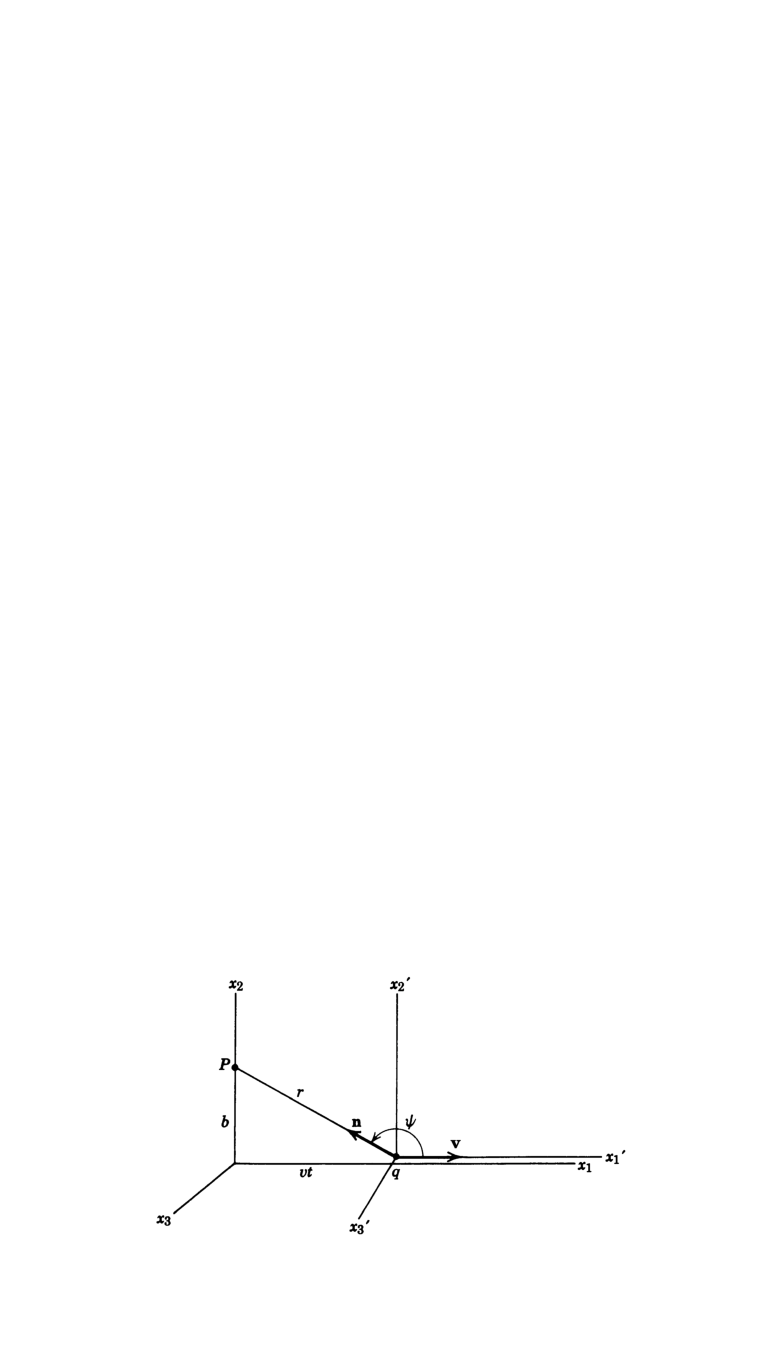
\includegraphics{11-8}
\caption{(Jackson Fig.~11.8) Particle of charge $q$ moving at constant velocity $\vv$ passes an observation point $P$ at impact parameter $b$.}
\label{11.8}
\end{figure}

\begin{problem} \label{2.a}
	For the geometry of Fig.~\ref{11.8} the coordinates of $P$ and $q$ at a common time in $K$ can be written $\xap = (ct, \vbb)$, $\xaq = (ct, \vv t)$, with $\vbb \vdot \vv = 0$.  By considering the general form of $\Fab$ in the rest frame of the charge, show that
	\beqn \label{show2.a}
		\Fab = \frac{q}{c} \frac{\Xa \Ub - \Xb \Ua}{[(\Usa \Xa / c)^2 - \Xsa \Xa]^{3/2}}.
	\eeqn
	Verify that this yields the expressions
	\begin{align} \label{fields}
		\Eq &= \Eq' = -\frac{q \gam v t}{(b^2 + \gam^2 v^2 t^2)^{3/2}}, &
		\Ew &= \gam \Ew' = \frac{\gam q b}{(b^2 + \gam^2 v^2 t^2)^{3/2}}, &
		\Be &= \gam \bet \Ew' = \bet \Ew,
	\end{align}
	with all other components vanishing, in the inertial frame $K$.
\end{problem}


\newcommand{\Fmat}{\mqty[	0 & -\Eq & -\Ew & -\Ee \\
						\Eq & 0 & -\Be & \Bw \\
						\Ew & \Be & 0 & -\Bq \\
						\Ee & -\Bw & \Bq & 0 ]}
\newcommand{\Fpab}{{F'}^{\alp\bet}}
\newcommand{\rp}{{r'}}
\newcommand{\tLam}{\tilde{\Lam}}
\newcommand{\Lammat}{\mqty[\gam & \gam \beta & 0 & 0 \\	
						\gam \beta & \gam & 0 & 0 \\
						0 & 0 & 1 & 0 \\
						0 & 0 & 0 & 1 ]}

\begin{solution}
	From Jackson~(11.137),
	\beqn \label{F}
		\Fab = \Fmat,
	\eeqn
	and from the equation immediately preceding Jackson~(11.151),
	\begin{align*}
		\Eq' &= -\frac{q v t'}{\rp^3}, &
		\Ew' &= \frac{q b}{\rp^3}, &
		\Ee' &= 0, &
		\Bq' &= 0, &
		\Bw' &= 0, &
		\Be' &= 0,
	\end{align*}
	in the rest frame of the charge for the geometry in Fig.~\ref{1}.  Here, $r' = \sqrt{b^2 + v^2 {t'}^2}$.  Then, in $K'$,
	\beqn \label{thing2.1b}
		\Fpab = \frac{q}{(b^2 + v^2 {t'}^2)^{3/2}}
			\mqty[0 & v t' & -b & 0 \\
				-v t' & 0 & 0 & 0 \\
				b & 0 & 0 & 0 \\
				0 & 0 & 0 & 0 ].
	\eeqn
	Now we will boost into the frame $K$.  From Jackson~(11.147), $F' = \Lam F \tLam$, although we need $F = \Lam F' \tLam$, where we boost in the direction opposite the particle's motion.  According to Jackson~(11.113), the Lorentz boost in the $-x'$ direction is
	\beqn \label{Lam2}
		\Lam = \Lammat.
	\eeqn
	Then
	\begin{align*}
		\Fab &= \frac{q}{(b^2 + v^2 {t'}^2)^{3/2}} \Lammat
			\mqty[ 0 & v t' & -b & 0 \\
				-v t' & 0 & 0 & 0 \\
				b & 0 & 0 & 0 \\
				0 & 0 & 0 & 0 ]
			\Lammat \\
		&= \frac{q}{(b^2 + v^2 {t'}^2)^{3/2}}
			\mqty[ -\gam \bet v t' & \gam v t' & -\gam b & 0 \\
				-\gam v t' & \gam \bet v t' & -\gam \bet b & 0 \\
				b & 0 & 0 & 0 \\
				0 & 0 & 0 & 0 ]
			\Lammat
		= \frac{q}{(b^2 + v^2 {t'}^2)^{3/2}}
			\mqty[ 0 & v t' & -\gam b & 0 \\
				-v t' & 0 & -\gam \bet b & 0 \\
				\gam b & \gam \bet b & 0 & 0 \\
				0 & 0 & 0 & 1 ].
	\end{align*}
	From \refeq{lorentz}, $t' = \gam t$ since $x = 0$.  Finally,
	\beqn \label{thing2.1}
		\Fab = \frac{\gam q}{(b^2 + \gam^2 v^2 t^2)^{3/2}} 
			\mqty[0 & v t & -b & 0 \\
				-v t & 0 & -v b / c & 0 \\
				b & v b / c & 0 & 0 \\
				0 & 0 & 0 & 0 ].
	\eeqn
	
	Now we will begin from \refeq{show2.a} and find $\Fab$ directly in $K$.  In accordance with Fig.~\ref{11.8},
	\begin{align*}
		\Xa &= (0, \vbb - \vv t) = (0, -v t, b, 0), &
		\Ua &= \gam (c, \vv) = \gam (c, v, 0, 0),
	\end{align*}
	and so
	\beq
		\Xa \Ub - \Xb \Ua = \gam
			\mqty[ 0 & 0 & 0 & 0 \\
				-c v t & -v^2 t & 0 & 0 \\
				c b & v b & 0 & 0 \\
				0 & 0 & 0 & 0 ]
		- \gam
			\mqty[ 0 & -c v t & c b & 0 \\
				0 & -v^2 t & v b & 0 \\
				0 & 0 & 0 & 0 \\
				0 & 0 & 0 & 0 ]
		= \gam
			\mqty[0 & c v t & - c b & 0 \\
				-c v t & 0 & -v b & 0 \\
				c b & v b & 0 & 0 \\
				0 & 0 & 0 & 0 ].
	\eeq
	Additionally,
	\begin{align*}
		\Usa \Xa &= \gam \mqty[ c & -v & 0 & 0 ] \mqty[ 0 \\ -v t \\ b \\ 0 ]
		= \gam v^2 t, &
		\Xsa \Xa &= \mqty[ 0 & vt & -b & 0 ] \mqty[ 0 \\ -v t \\ b \\ 0 ]
		= -v^2 t^2 - b^2.
	\end{align*}
	Then, applying \refeq{show2.a},
	\beq
		\Fab = \frac{\gam q}{(\gam^2 v^4 t^2 / c^2 + v^2 t^2 + b^2)^{3/2}}
			\mqty[0 & v t & -b & 0 \\
				-v t & 0 & -v b / c & 0 \\
				b & v b / c & 0 & 0 \\
				0 & 0 & 0 & 0 ].
	\eeq
	Note that
	\beq
		v^2 t^2 + \frac{\gam^2 v^4 t^2}{c^2} = v^2 t^2 \left( 1 + \gam^2 \frac{v^2}{c^2} \right)
		= v^2 t^2 \left( 1 + \frac{\bet^2}{1 - \bet^2} \right)
		= v^2 t^2 \frac{1 - \bet^2 + \bet^2}{1 - \bet^2}
		= \gam^2 v^2 t^2,
	\eeq
	so we have again arrived at \refeq{thing2.1}.  Thus, we have proven \refeq{show2.a}.
	
	In addition, comparing \refeq{thing2.1} with \refeq{F}, we see that
	\begin{align*}
		\Eq &= -\frac{q \gam v t}{(b^2 + \gam^2 v^2 t^2)^{3/2}}, &
		\Ew &= \frac{\gam q b}{(b^2 + \gam^2 v^2 t^2)^{3/2}}, &
		\Be &= \frac{\gam \bet q b}{(b^2 + \gam^2 v^2 t^2)^{3/2}} = \bet \Ew.
	\end{align*}
	Comparing \refeq{thing2.1b} with \refeq{F} as well, and making the substitution $t' = \gam t$, yields
	\begin{align*}
		\Eq' &= -\frac{q \gam v t}{(b^2 + \gam^2 v^2 t^2)^{3/2}}, &
		\Ew' &= \frac{q b}{(b^2 + \gam^2 v^2 t^2)^{3/2}},
	\end{align*}
	so we have also verified \refeq{fields}. \qed
\end{solution}


\newcommand{\xpap}{{x'}^\alp_p}
\newcommand{\xpaq}{{x'}^\alp_q}
\newcommand{\Ya}{Y^\alp}
\newcommand{\Ysa}{Y_\alp}
\newcommand{\Yb}{Y^\bet}
\newcommand{\Ypa}{{Y'}^\alp}

\begin{problem}
	Repeat the calculation, using as the starting point the common-time coordinates in the rest frame, ${\xpap = (ct', \vbb - \vv t')}$ and $\xpaq = (ct', 0)$.  Show that
	\beqn \label{show2.b}
		\Fab = \frac{q}{c} \frac{\Ya \Ub - \Yb \Ua}{(- \Ysa \Ya)^{3/2}},
	\eeqn
	where $\Ypa = \xpap - \xpaq$.  Verify that the fields are the same as in \ref{2.a}.  Note that to obtain the results of \refeq{fields} it is necessary to use the time $t$ of the observation point $P$ in $K$ as the time parameter.
\end{problem}

\newcommand{\Ypsa}{{Y'}_\alp}
\newcommand{\Ypb}{{Y'}^\bet}
\newcommand{\Upa}{{U'}^\alp}
\newcommand{\Upb}{{U'}^\bet}
\newcommand{\vo}{\mathbf{0}}
\newcommand{\tp}{{t'}}

\begin{solution}
	Firstly, note that
	\begin{align*}
		\Ypa &= (0, \vbb - \vv t') = (0, -v t', b, 0), &
		\Upa &= (c, \vo) = (c, 0, 0, 0),
	\end{align*}
	Then
	\beq
		\Ypa \Upb - \Ypb \Upa = c
			\mqty[ 0 & 0 & 0 & 0 \\
				-v t' & 0 & 0 & 0 \\
				b & 0 & 0 & 0 \\
				0 & 0 & 0 & 0 ]
		- c
			\mqty[ 0 & -v t' & b & 0 \\
				0 & 0 & 0 & 0 \\
				0 & 0 & 0 & 0 \\
				0 & 0 & 0 & 0 ]
		= c
			\mqty[ 0 & v t' & -b & 0 \\
				-v t' & 0 & 0 & 0 \\
				b & 0 & 0 & 0 \\
				0 & 0 & 0 & 0 ],
	\eeq
	and
	\beq
		\Ypsa \Ypa = \mqty[ 0 & v t' & -b & 0 ] \mqty[ 0 \\ -v t' \\ b \\ 0 ] = -v^2 \tp^2 - b^2,
	\eeq
	so, from \refeq{show2.b}, in $K'$ we have
	\beq
		\Fpab = \frac{q}{(b^2 + v^2 \tp^2)^{3/2}}
			\mqty[ 0 & v t' & -b & 0 \\
				-v t' & 0 & 0 & 0 \\
				b & 0 & 0 & 0 \\
				0 & 0 & 0 & 0 ],
	\eeq
	which is identical to \refeq{thing2.1b}.  We know that boosting into $K$ yields \refeq{thing2.1}.
	
	Now we will find $\Fab$ directly in $K$ by boosting $\Ypa$ and $\Upa$.  From Jackson~(11.84), $x' = \Lam x$ (where $x$ represents $x^\alp$), and we once again use $\Lam$ given by \refeq{Lam2} to perform $x = \Lam x'$.  We obtain
	\begin{align*}
		Y &= \Lam Y'
		= \Lammat \mqty[ 0 \\ -v t' \\ b \\ 0]
		= \mqty[ -\gam \bet v t' \\ -\gam v t' \\ b \\ 0 ], &
		U &= \Lam U'
		= \Lammat \mqty[ c \\ 0 \\ 0 \\ 0 ]
		= \gam c \mqty[ 1 \\ \bet \\ 0 \\ 0 ].
	\end{align*}
	Then
	\beq
		\Ya \Ub - \Yb \Ua = \gam c
			\mqty[ -\gam \bet v t' & -\gam \bet^2 v t' & 0 & 0 \\
				-\gam v t' & -\gam \bet v t' & 0 & 0 \\
				b & \bet b & 0 & 0 \\
				0 & 0 & 0 & 0 ]
			- \gam c
			\mqty[ -\gam \bet v t' & -\gam v t' & b & 0 \\
				-\gam \bet^2 v t' & -\gam \bet v t' & \bet b & 0 \\
				0 & 0 & 0 & 0 \\
				0 & 0 & 0 & 0 ]
		= c
			\mqty[ 0 & v t' & -\gam b & 0 \\
				-v t' & 0 & -\gam \bet b & 0 \\
				\gam b & \gam \bet b & 0 & 0 \\
				0 & 0 & 0 & 0 ],
	\eeq
	and
	\beq
		\Ysa \Ya = \mqty[ -\gam \bet v t' & \gam v t' & -b & 0] \mqty[ -\gam \bet v t' \\ -\gam v t' \\ b \\ 0 ]
		= \gam^2 \bet^2 v^2 \tp^2 - \gam^2 v^2 \tp^2 - b^2
		= -v^2 \tp^2 - b^2.
	\eeq
	Making these substitutions into \refeq{show2.b}, and using $t' = \gam t$,
	\beq
		\Fab = \frac{q}{(b^2 + v^2 \tp^2)^{3/2}}
			\mqty[ 0 & v t' & -\gam b & 0 \\
				-v t' & 0 & -\gam v b / c & 0 \\
				\gam b & \gam v b / c & 0 & 0 \\
				0 & 0 & 0 & 0 ]
		= \frac{\gam q}{(b^2 + \gam^2 v^2 t^2)^{3/2}}
			\mqty[ 0 & v t & -b & 0 \\
				-v t & 0 & -v b / c & 0 \\
				b & v b / c & 0 & 0 \\
				0 & 0 & 0 & 0 ],
	\eeq
	which is identical to \refeq{thing2.1}, and therefore gives the fields from \refeq{fields} as in \ref{2.a}.  Thus, we have proven \refeq{show2.b}. \qed
\end{solution}


\newcommand{\Za}{Z^\alp}
\newcommand{\Zsa}{Z_\alp}
\newcommand{\Zb}{Z^\bet}
\newcommand{\vbet}{\boldsymbol{\beta}}

\begin{problem}
	Finally, consider the coordinate $\xap = (ct, \vbb)$ and the ``retarded-time'' coordinate $\xaq = [ct - R, \vbet(ct - R)]$ where $R$ is the distance between $P$ and $q$ at the retarded time.  Define the difference as $\Za = [R, \vbb - \vbet(ct - R)]$.  Show that in terms of $\Za$ and $\Ua$ the field is
	\beqn \label{show2.c}
		\Fab = \frac{q}{c} \frac{\Za \Ub - \Zb \Ua}{(\Usa \Za / c)^3}.
	\eeqn
\end{problem}
\vfix

\begin{solution}
	Referring to Fig~\ref{11.8},
	\begin{align*}
		\Za &= (R, \vbb - \vv t + \vv R / c) = [R, -v (t - R / c), b, 0], &
		\Ua &= \gam (c, \vv) = \gam (c, v, 0, 0).
	\end{align*}
	Then
	\begin{align*}
		\Za\Ub - \Zb \Ua &= \gam
			\mqty[c R & R v & 0 & 0 \\
				-v (c t - R) & -v^2 (t - R / c) & 0 & 0 \\
				c b & b v & 0 & 0 \\
				0 & 0 & 0 & 0 ]
			- \gam
			\mqty[ c R & -v (c t - R) & c b & 0 \\
				R v & -v^2 (t - R / c) & b v & 0 \\
				0 & 0 & 0 & 0 \\
				0 & 0 & 0 & 0 ] \\
		&= \gam c
			\mqty[0 & v t & -b & 0 \\
				-v t & 0 & -v b / c & 0 \\
				b & v b / c & 0 & 0 \\
				0 & 0 & 0 & 0 ],
	\end{align*}
	and
	\beq
		\Usa \Za = \gam \mqty[ c & -v & 0 & 0 ] \mqty[ R \\ -v (t - R / c) \\ b \\ 0 ]
		= \gam cR + \gam v^2(t - R/c),
	\eeq
	so
	\beq
		\frac{\Usa \Za}{c} = \gam R + \gam \bet^2 c t - \gam \bet^2 R
		= (1 - \bet^2) \gam R + \gam \bet^2 c t
		= \frac{R}{\gam} + \gam \bet^2 c t.
	\eeq
	
	Note that $\xap$ and $\xaq$, as they are defined here, have lightlike separation since $R / c$ is, by definition, the time it takes light to travel from $\xaq$ to $\xap$.  Then
	\beq
		0 = \Zsa \Za
		= \mqty[ R & v (t - R / c) & -b & 0 ] \mqty[ R \\ -v (t - R / c) \\ b \\ 0 ]
		= R^2 - v^2 (t - R / c)^2 - b^2,
	\eeq
	which implies
	\beq
		R^2 = b^2 + v^2 (t - R / c)^2.
	\eeq
	This is corroborated by the geometry of Fig.~\ref{11.8}, since $t - R / c$ is the retarded time.  Then, referring to the denominator of \refeq{thing2.1}, we find
	\begin{align*}
		b^2 + \gam^2 v^2 t^2 &= R^2 - v^2 (t - R / c)^2 + \gam^2 v^2 t^2
		= R^2 - \bet^2  (c^2 t^2 - 2 R c t + R^2) + \gam^2 \bet^2 c^2 t^2 \\
		&= (1 - \bet^2) R^2 + 2 R \bet^2 c t + (\gam^2 - 1) \bet^2 c^2 t^2
		= \frac{R^2}{\gam^2} + 2 R \bet^2 c t + \gam^2 \bet^4 c^2 t^2
		= \left( \frac{R}{\gam} + \gam \bet^2 c t \right)^2 \\
		&= \left( \frac{\Usa \Za}{c} \right)^2.
	\end{align*}
	In summary, we have found
	\beq
		\Fab = \frac{\gam q}{(b^2 + \gam^2 v^2 t^2)^{3/2}}
			\mqty[0 & v t & -b & 0 \\
				-v t & 0 & -v b / c & 0 \\
				b & v b / c & 0 & 0 \\
				0 & 0 & 0 & 0 ],
	\eeq
	which is identical to \refeq{thing2.1}.  Thus, we have proven \refeq{show2.c}. \qed
\end{solution}



\vfill
In addition to the course lecture notes, I consulted Jackson's \emph{Classical Electrodynamics} while writing up these solutions.
\end{document}